\documentclass[aspectratio=169,10pt]{beamer}

\usepackage[T1]{fontenc}
\usepackage{lmodern}
\usepackage{amsmath,amssymb,mathtools}
\usepackage{booktabs}
\usepackage{array}
\usepackage{tabularx}
\usepackage{listings}
\usepackage{tikz}
\usetikzlibrary{arrows.meta,positioning,calc,fit,shapes.misc}

% ---------- Palette and typography ----------
\definecolor{CrisNavy}{HTML}{17233C}
\definecolor{CrisBlue}{HTML}{3568D4}
\definecolor{CrisLightBlue}{HTML}{EAF0FC}
\definecolor{CrisAmber}{HTML}{E99A35}
\definecolor{CrisLightAmber}{HTML}{FFF1DE}
\definecolor{CrisGreen}{HTML}{268A73}
\definecolor{CrisLightGreen}{HTML}{E4F4EF}
\definecolor{CrisRed}{HTML}{C84A54}
\definecolor{CrisLightRed}{HTML}{FBEAEC}
\definecolor{CrisInk}{HTML}{202736}
\definecolor{CrisMuted}{HTML}{657084}
\definecolor{CrisPaper}{HTML}{FBFAF7}

\setbeamercolor{normal text}{fg=CrisInk,bg=CrisPaper}
\setbeamercolor{structure}{fg=CrisBlue}
\setbeamercolor{frametitle}{fg=CrisNavy,bg=CrisPaper}
\setbeamercolor{title}{fg=white,bg=CrisNavy}
\setbeamercolor{subtitle}{fg=CrisLightBlue,bg=CrisNavy}
\setbeamercolor{block title}{fg=white,bg=CrisBlue}
\setbeamercolor{block body}{fg=CrisInk,bg=CrisLightBlue}
\setbeamercolor{block title alerted}{fg=white,bg=CrisRed}
\setbeamercolor{block body alerted}{fg=CrisInk,bg=CrisLightRed}
\setbeamercolor{block title example}{fg=white,bg=CrisGreen}
\setbeamercolor{block body example}{fg=CrisInk,bg=CrisLightGreen}

\setbeamerfont{title}{series=\bfseries,size=\LARGE}
\setbeamerfont{subtitle}{size=\large}
\setbeamerfont{frametitle}{series=\bfseries,size=\Large}
\setbeamerfont{block title}{series=\bfseries}

\setbeamertemplate{navigation symbols}{}
\setbeamertemplate{itemize item}{\color{CrisBlue}$\blacktriangleright$}
\setbeamertemplate{itemize subitem}{\color{CrisAmber}$\bullet$}
\setbeamertemplate{enumerate item}{\color{CrisBlue}\bfseries\insertenumlabel.}
\setbeamertemplate{frametitle}{%
  \vspace{0.35em}\insertframetitle\par
  \vspace{-0.55em}{\color{CrisBlue}\rule{\textwidth}{0.8pt}}
}
\setbeamertemplate{footline}{%
  \leavevmode%
  \hbox{%
    \begin{beamercolorbox}[wd=.82\paperwidth,ht=2.7ex,dp=1.1ex,leftskip=1.2em]{author in head/foot}%
      \color{CrisMuted}\scriptsize From Cells to Memory \hspace{0.6em}|\hspace{0.6em} CRIS Workshop
    \end{beamercolorbox}%
    \begin{beamercolorbox}[wd=.18\paperwidth,ht=2.7ex,dp=1.1ex,rightskip=1.2em plus1fil]{date in head/foot}%
      \hfill\color{CrisMuted}\scriptsize\insertframenumber
    \end{beamercolorbox}%
  }%
}

\lstdefinestyle{criscode}{
  basicstyle=\ttfamily\small,
  keywordstyle=\color{CrisBlue}\bfseries,
  commentstyle=\color{CrisMuted}\itshape,
  stringstyle=\color{CrisGreen},
  showstringspaces=false,
  columns=fullflexible,
  keepspaces=true,
  frame=single,
  rulecolor=\color{CrisLightBlue},
  backgroundcolor=\color{white},
  xleftmargin=0.4em,
  xrightmargin=0.4em,
  aboveskip=0.4em,
  belowskip=0.4em
}

% ---------- Notation used only in this talk ----------
\newcommand{\Sep}{\mathbin{*}}
\newcommand{\AuthM}[1]{\mathsf{Auth}_{\gamma_m}(#1)}
\newcommand{\AuthC}[1]{\mathsf{Auth}_{\gamma_c}(#1)}
\newcommand{\Snap}[1]{\mathsf{Snap}_{\gamma_c}(#1)}
\newcommand{\ptfull}[2]{#1\mathrel{\mapsto_{\gamma_m}}#2}
\newcommand{\ptfrac}[3]{#1\mathrel{\mapsto_{\gamma_m}^{#2}}#3}
\newcommand{\ptro}[2]{#1\mathrel{\mapsto_{\gamma_m}^{\Box}}#2}
\newcommand{\upd}{\mathrel{\leadsto}}
\newcommand{\code}[1]{\texttt{\detokenize{#1}}}
\newcommand{\api}[1]{\textcolor{CrisMuted}{\scriptsize\texttt{\detokenize{#1}}}}
\newcommand{\good}[1]{\textcolor{CrisGreen}{#1}}
\newcommand{\warn}[1]{\textcolor{CrisRed}{#1}}
\newcommand{\keypoint}[1]{\textcolor{CrisBlue}{\bfseries #1}}

\title{From Cells to Memory}
\subtitle{Protocols as Resources in CRIS}
\author{Presenter name}
\institute{Program Verification Workshop}
\date{29 July 2026}

\begin{document}

% 1 -- 0:00
\begin{frame}[plain]
  \begin{tikzpicture}[remember picture,overlay]
    \fill[CrisNavy] (current page.south west) rectangle (current page.north east);
    \fill[CrisBlue] (current page.south west) rectangle ([yshift=0.23\paperheight]current page.south east);
    \draw[CrisAmber,line width=3pt] ([xshift=0.08\paperwidth,yshift=-0.30\paperheight]current page.north west)
      -- ([xshift=0.92\paperwidth,yshift=-0.30\paperheight]current page.north west);
  \end{tikzpicture}
  \vspace{1.4cm}
  \begin{center}
    {\usebeamerfont{title}\color{white}\inserttitle\par}
    \vspace{0.3cm}
    {\usebeamerfont{subtitle}\color{CrisLightBlue}\insertsubtitle\par}
    \vspace{1.0cm}
    {\large\color{white}A memory map, shared reads, frozen facts, and snapshots of the past\par}
    \vfill
    {\small\color{white}\insertauthor\quad\textbullet\quad\insertdate}
  \end{center}
\end{frame}

% 2 -- 0:30
\begin{frame}{Where this talk starts}
  \begin{center}
  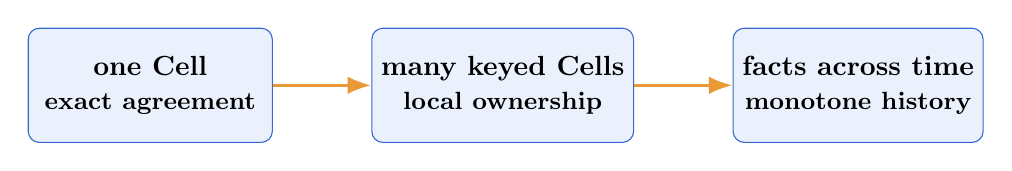
\begin{tikzpicture}[
    node distance=1.25cm,
    box/.style={rounded corners,draw=CrisBlue,fill=CrisLightBlue,minimum width=3.1cm,minimum height=1.45cm,align=center,font=\bfseries},
    arr/.style={-{Latex[length=3mm]},very thick,CrisAmber}
  ]
    \node[box] (cell) {one Cell\\\small exact agreement};
    \node[box,right=of cell] (map) {many keyed Cells\\\small local ownership};
    \node[box,right=of map] (time) {facts across time\\\small monotone history};
    \draw[arr] (cell) -- (map);
    \draw[arr] (map) -- (time);
  \end{tikzpicture}
  \end{center}

  \vspace{0.45cm}
  From the preceding Cell example, keep only three ideas:
  \begin{itemize}
    \item the client owns a \keypoint{capability} such as \(\mathsf{cell}(v)\),
    \item the module retains a matching \keypoint{authoritative view}, and
    \item global validity makes their claims compatible.
  \end{itemize}

  \begin{block}{Today}
    Scale that pattern from one slot to a memory, then change the compatibility relation from
    “equal now” to “no smaller than a past observation.”
  \end{block}
\end{frame}

% 3 -- 2:30
\begin{frame}{The promise}
  By the end, you should be able to:

  \vspace{0.3cm}
  \begin{columns}[T,onlytextwidth]
    \column{0.31\textwidth}
      \begin{block}{Read}
        Read the four memory rules and tell which resource crosses each call boundary.
      \end{block}
    \column{0.31\textwidth}
      \begin{block}{Predict}
        Predict what an update changes---and what it preserves automatically.
      \end{block}
    \column{0.31\textwidth}
      \begin{block}{Choose}
        Choose a standard resource algebra from the protocol a client needs.
      \end{block}
  \end{columns}

  \vspace{0.55cm}
  \begin{center}
    \Large\bfseries\color{CrisNavy}
    Start from the protocol, not from the algebraic carrier.
  \end{center}
\end{frame}

% 4 -- 4:00
\begin{frame}{Protocols already hide in ordinary programs}
  \begin{columns}[T,onlytextwidth]
    \column{0.48\textwidth}
      \begin{block}{Key--value ownership}
        “I may access key \(k\), and it currently contains \(v\).”
      \end{block}
      \begin{block}{Shared immutable access}
        “Several clients may read; nobody may write until the shares return.”
      \end{block}
    \column{0.48\textwidth}
      \begin{block}{Publication / freeze}
        “This final result may be copied forever and can no longer change.”
      \end{block}
      \begin{block}{Monotonic history}
        “A later observation cannot be smaller than this past one.”
      \end{block}
  \end{columns}

  \vspace{0.25cm}
  \begin{exampleblock}{Thirty-second prompt}
    Name another real program protocol as: \emph{a capability} + \emph{an allowed transition}.
  \end{exampleblock}
\end{frame}

% 5 -- 7:00
\begin{frame}[fragile]{Running example: a one-cell allocation}
  \begin{columns}[T,onlytextwidth]
    \column{0.52\textwidth}
\begin{lstlisting}[style=criscode]
p = Mem.alloc(1);
Mem.store(p, 7);
x = Mem.load(p);
Mem.free(p);
\end{lstlisting}
      \small
      The concrete module keeps a private heap and implements these operations with internal state
      reads and writes.

    \column{0.44\textwidth}
      \begin{alertblock}{The modularity question}
        What prevents an unknown component from storing through \code{p} between our store and load?
      \end{alertblock}
      \vspace{0.35cm}
      \begin{center}
        \Large “We inspected all its code”\\[0.15cm]
        \warn{is not a modular answer.}
      \end{center}
  \end{columns}

  \vfill
  \scriptsize The checked-in implementation's \code{free} removes one cell, so the main example uses \code{alloc(1)}.
\end{frame}

% 6 -- 9:00
\begin{frame}{The client-facing memory contract}
  Read \(\ptfull{\ell}{v}\) as: “I own access to \(\ell\), whose current value is \(v\).”

  \vspace{0.35cm}
  \renewcommand{\arraystretch}{1.35}
  \begin{tabularx}{\textwidth}{>{\bfseries}l X X}
    \toprule
    operation & required resource & returned resource / fact \\
    \midrule
    \code{alloc(n)} & valid size & fresh region \(\ptfull{\ell+i}{\mathsf{undef}}\) \\
    \code{load(l)} & \(\ptfrac{\ell}{q}{v}\) & \(\mathsf{ret}=v\) and the same fraction \\
    \code{store(l,w)} & full \(\ptfull{\ell}{v}\) & full \(\ptfull{\ell}{w}\) \\
    \code{free(l)} & full \(\ptfull{\ell}{v}\) & resource consumed \\
    \bottomrule
  \end{tabularx}

  \vspace{0.45cm}
  \begin{block}{A call boundary transfers capabilities}
    The precondition tells the module what the caller authorizes; the postcondition tells the caller
    what capability comes back.
  \end{block}
\end{frame}

% 7 -- 14:00
\begin{frame}{Why not expose one global heap fact?}
  \begin{columns}[T,onlytextwidth]
    \column{0.46\textwidth}
      \begin{alertblock}{Global, fragile}
        \[
          \mathsf{heap}=M
        \]
        A store anywhere changes the assertion. Every client must reason about the whole map again.
      \end{alertblock}
    \column{0.50\textwidth}
      \begin{exampleblock}{Local, stable}
        \[
          \ptfull{\ell}{7}\Sep\ptfull{k}{20}
        \]
        A store at \(\ell\) should preserve the framed fact about \(k\):
        \[
          \ptfull{\ell}{8}\Sep\ptfull{k}{20}.
        \]
      \end{exampleblock}
  \end{columns}

  \vspace{0.4cm}
  \begin{center}
    \Large\bfseries\color{CrisNavy}
    Give each client exactly the entry it may rely on.
  \end{center}
\end{frame}

% 8 -- 17:00
\begin{frame}{A memory is a map of Cells}
  \begin{center}
  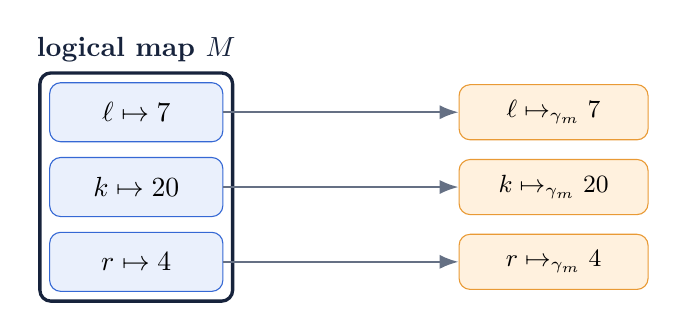
\begin{tikzpicture}[
    cell/.style={draw=CrisBlue,fill=CrisLightBlue,rounded corners,minimum width=2.2cm,minimum height=0.75cm,align=center},
    token/.style={draw=CrisAmber,fill=CrisLightAmber,rounded corners,minimum width=2.4cm,minimum height=0.7cm,align=center,font=\small\bfseries},
    arr/.style={-{Latex[length=2.4mm]},thick,CrisMuted}
  ]
    \node[cell] (a) at (0,1.3) {\(\ell \mapsto 7\)};
    \node[cell] (b) at (0,0.35) {\(k \mapsto 20\)};
    \node[cell] (c) at (0,-0.6) {\(r \mapsto 4\)};
    \node[draw=CrisNavy,very thick,rounded corners,fit=(a)(b)(c),label={[CrisNavy]above:\bfseries logical map \(M\)}] (map) {};

    \node[token] (ta) at (5.3,1.3) {\(\ptfull{\ell}{7}\)};
    \node[token] (tb) at (5.3,0.35) {\(\ptfull{k}{20}\)};
    \node[token] (tc) at (5.3,-0.6) {\(\ptfull{r}{4}\)};
    \draw[arr] (a.east) -- (ta.west);
    \draw[arr] (b.east) -- (tb.west);
    \draw[arr] (c.east) -- (tc.west);
  \end{tikzpicture}
  \end{center}

  \vspace{0.35cm}
  \begin{block}{\code{ghost_map} packages the repeated Cell pattern}
    One authoritative view of the whole dictionary; independent points-to-like fragments for keys.
  \end{block}

  \scriptsize Artifact note: \code{MemA.v} manually builds an equivalent map. CRIS also has a compatible interface in \code{CRIS/theories/iris_system/lib/ghost_map.v}, but current \code{MemA} does not use it.
\end{frame}

% 9 -- 19:00
\begin{frame}{Two views of one logical map}
  \begin{columns}[T,onlytextwidth]
    \column{0.47\textwidth}
      \begin{block}{Module view}
        \[
          \AuthM{M}
        \]
        \begin{itemize}
          \item authoritative view of the whole map,
          \item kept at full fraction inside the module proof,
          \item ghost state---not the physical heap.
        \end{itemize}
      \end{block}
    \column{0.49\textwidth}
      \begin{block}{Client view}
        \[
          \ptfrac{\ell}{q}{v}
        \]
        \begin{itemize}
          \item fragment for one key,
          \item carries value knowledge and permission,
          \item the ghost name \(\gamma_m\) links both views.
        \end{itemize}
      \end{block}
  \end{columns}

  \vspace{0.45cm}
  \begin{center}
    \large One physical location, one logical entry, two compatible ownership views.
  \end{center}
\end{frame}

% 10 -- 22:00
\begin{frame}{The one law to remember}
  \vspace{0.7cm}
  \begin{center}
    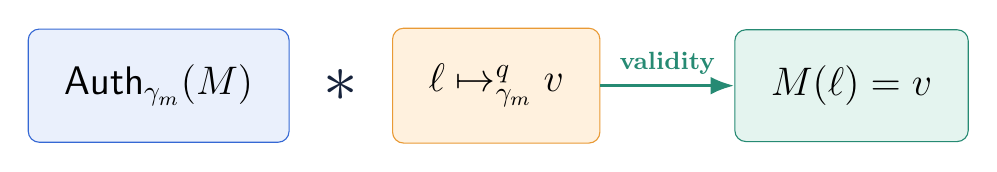
\begin{tikzpicture}
      \node[draw=CrisBlue,fill=CrisLightBlue,rounded corners,inner sep=13pt,font=\Large] (auth) {\(\AuthM{M}\)};
      \node[draw=CrisAmber,fill=CrisLightAmber,rounded corners,inner sep=13pt,font=\Large,right=1.3cm of auth] (frag) {\(\ptfrac{\ell}{q}{v}\)};
      \node[font=\Huge,CrisNavy] at ($(auth.east)!0.5!(frag.west)$) {\(*\)};
      \node[draw=CrisGreen,fill=CrisLightGreen,rounded corners,inner sep=13pt,font=\Large,right=1.7cm of frag] (fact) {\(M(\ell)=v\)};
      \draw[-{Latex[length=3mm]},very thick,CrisGreen] (frag.east) -- node[above,font=\small\bfseries]{validity} (fact.west);
    \end{tikzpicture}
  \end{center}

  \vspace{0.8cm}
  \begin{itemize}
    \item Validity checks whether all simultaneously owned claims can coexist.
    \item A client cannot forge \(\ptfull{\ell}{w}\) when authority records \(v\neq w\).
    \item For a different key, a fragment imposes a different, independent lookup constraint.
  \end{itemize}

  \vfill
  \api{ghost_map_lookup}
\end{frame}

% 11 -- 25:00
\begin{frame}{Where authority lives: the CRIS IST}
  \begin{columns}[T,onlytextwidth]
    \column{0.64\textwidth}
      \begin{block}{Simplified module-local invariant}
      \[
      \begin{aligned}
      \mathsf{IST}(st_A,st_I)\;\triangleq\;\exists m,M.\;&
        st_I[\code{Mem.mem}]=m \\
        &{}\Sep \ulcorner\mathsf{repr}(m)=M\urcorner \\
        &{}\Sep \AuthM{M}
      \end{aligned}
      \]
      \end{block}
      \small
      At each simulation interaction point, the private concrete heap and the authoritative logical map agree.

    \column{0.32\textwidth}
      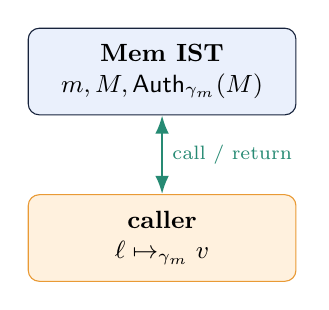
\begin{tikzpicture}[
        box/.style={rounded corners,minimum width=3.4cm,minimum height=1.1cm,align=center,font=\small\bfseries},
        arr/.style={<->,>=Latex,thick,CrisGreen}
      ]
        \node[box,draw=CrisNavy,fill=CrisLightBlue] (ist) {Mem IST\\\(m,M,\AuthM{M}\)};
        \node[box,draw=CrisAmber,fill=CrisLightAmber,below=1.0cm of ist] (client) {caller\\\(\ptfull{\ell}{v}\)};
        \draw[arr] (ist) -- node[right,font=\scriptsize]{call / return} (client);
      \end{tikzpicture}
  \end{columns}

  \vspace{0.25cm}
  \begin{exampleblock}{Boundary discipline}
    A method combines hidden authority with the caller's fragment, restores the IST, and returns the promised fragment.
  \end{exampleblock}
\end{frame}

% 12 -- 29:00
\begin{frame}{The packaged rules are the protocol}
  \small
  \renewcommand{\arraystretch}{1.38}
  \begin{tabularx}{\textwidth}{>{\bfseries}l X l}
    \toprule
    logical operation & resource transition / consequence & needed permission \\
    \midrule
    lookup & \(\AuthM{M}\Sep\ptfrac{\ell}{q}{v}\;\Rightarrow\;M(\ell)=v\) & any compatible fractions \\
    insert & \(\AuthM{M}\upd\AuthM{M[\ell:=v]}\Sep\ptfull{\ell}{v}\) & full authority; fresh key \\
    update & \(\AuthM{M}\Sep\ptfull{\ell}{v}\upd\AuthM{M[\ell:=w]}\Sep\ptfull{\ell}{w}\) & full authority + full element \\
    delete & \(\AuthM{M}\Sep\ptfull{\ell}{v}\upd\AuthM{M\setminus\{\ell\}}\) & full authority + full element \\
    \bottomrule
  \end{tabularx}

  \vspace{0.45cm}
  \begin{center}
    \api{ghost_map_lookup}\quad
    \api{ghost_map_insert}\quad
    \api{ghost_map_update}\quad
    \api{ghost_map_delete}
  \end{center}

  \begin{block}{Notice what is absent}
    Clients never receive the authority. They receive only the fragment needed to authorize one entry's operation.
  \end{block}
\end{frame}

% 13 -- 33:00
\begin{frame}{Allocate: extend the map and create ownership}
  \vspace{0.45cm}
  \[
    \AuthM{M}
    \quad\upd\quad
    \AuthM{M[\ell:=\mathsf{undef}]}
      \Sep \ptfull{\ell}{\mathsf{undef}}
    \qquad \ell\notin\operatorname{dom}(M)
  \]

  \vspace{0.55cm}
  \begin{enumerate}
    \item The concrete allocator selects a fresh block/location.
    \item The proof extends the authoritative logical map at that same key.
    \item The new fragment crosses the call boundary to the client.
  \end{enumerate}

  \vspace{0.4cm}
  \begin{exampleblock}{Ownership is created at allocation time}
    Freshness is not just a numeric property of the address. It permits allocating a new compatible logical fragment.
  \end{exampleblock}

  \vfill
  \api{ghost_map_insert / ghost_map_insert_big}
\end{frame}

% 14 -- 36:00
\begin{frame}{Load: agreement without change}
  \begin{center}
  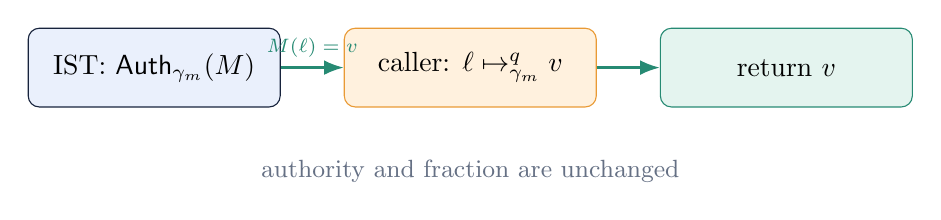
\begin{tikzpicture}[
    box/.style={rounded corners,draw,minimum width=3.2cm,minimum height=1.0cm,align=center},
    arr/.style={-{Latex[length=2.5mm]},thick}
  ]
    \node[box,draw=CrisNavy,fill=CrisLightBlue] (a) {IST: \(\AuthM{M}\)};
    \node[box,draw=CrisAmber,fill=CrisLightAmber,right=0.8cm of a] (f) {caller: \(\ptfrac{\ell}{q}{v}\)};
    \node[box,draw=CrisGreen,fill=CrisLightGreen,right=0.8cm of f] (r) {return \(v\)};
    \draw[arr,CrisGreen] (a) -- node[above,font=\scriptsize]{\(M(\ell)=v\)} (f);
    \draw[arr,CrisGreen] (f) -- (r);
    \node[font=\small,CrisMuted,below=0.55cm of f] {authority and fraction are unchanged};
  \end{tikzpicture}
  \end{center}

  \vspace{0.65cm}
  \begin{itemize}
    \item The fragment identifies the relevant entry and its value.
    \item The IST connects that logical entry to the concrete heap lookup.
    \item No knowledge of any other location is required.
  \end{itemize}

  \begin{block}{Read-only steps preserve every compatible frame}
    This is why any positive owned fraction---and later a persistent read-only fragment---can justify a load.
  \end{block}
\end{frame}

% 15 -- 39:00
\begin{frame}{Store: change exactly one entry}
  \vspace{0.4cm}
  \begin{align*}
    &\AuthM{\{\ell\!:\!7,\;k\!:\!20\}}
      \Sep \colorbox{CrisLightAmber}{\(\ptfull{\ell}{7}\)}
      \Sep \colorbox{CrisLightBlue}{\(\ptfull{k}{20}\)} \\
    &\hspace{4.5cm}\upd \\[0.2cm]
    &\AuthM{\{\ell\!:\!8,\;k\!:\!20\}}
      \Sep \colorbox{CrisLightAmber}{\(\ptfull{\ell}{8}\)}
      \Sep \colorbox{CrisLightBlue}{\(\ptfull{k}{20}\)}
  \end{align*}

  \vspace{0.45cm}
  \begin{columns}[T,onlytextwidth]
    \column{0.48\textwidth}
      \begin{exampleblock}{Changed}
        The authority and full fragment at \(\ell\) move together from 7 to 8.
      \end{exampleblock}
    \column{0.48\textwidth}
      \begin{block}{Framed}
        The token for \(k\) stays compatible and therefore remains untouched.
      \end{block}
  \end{columns}
\end{frame}

% 16 -- 42:00
\begin{frame}{One store proof, end to end}
  \small
  \begin{enumerate}
    \item \textbf{Open the IST}: obtain concrete heap \(m\), logical map \(M\), and \(\AuthM{M}\).
    \item \textbf{Check the entry}: combine authority with \(\ptfull{\ell}{v}\) to learn \(M(\ell)=v\), hence concrete lookup succeeds.
    \item \textbf{Execute}: step the concrete \code{SGet}/\code{SPut} implementation to heap \(m'\).
    \item \textbf{Update ghost state}: jointly obtain \(\AuthM{M[\ell:=w]}\Sep\ptfull{\ell}{w}\).
    \item \textbf{Close and return}: prove \(\mathsf{repr}(m')=M[\ell:=w]\), restore the IST, return the new fragment.
  \end{enumerate}

  \vspace{0.35cm}
  \begin{center}
  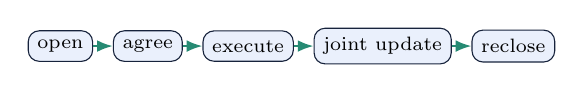
\begin{tikzpicture}[node distance=0.25cm, every node/.style={font=\scriptsize}, arr/.style={-{Latex[length=2mm]},CrisGreen,thick}]
    \node[draw=CrisNavy,fill=CrisLightBlue,rounded corners] (s1) {open};
    \node[draw=CrisNavy,fill=CrisLightBlue,rounded corners,right=of s1] (s2) {agree};
    \node[draw=CrisNavy,fill=CrisLightBlue,rounded corners,right=of s2] (s3) {execute};
    \node[draw=CrisNavy,fill=CrisLightBlue,rounded corners,right=of s3] (s4) {joint update};
    \node[draw=CrisNavy,fill=CrisLightBlue,rounded corners,right=of s4] (s5) {reclose};
    \draw[arr] (s1)--(s2); \draw[arr] (s2)--(s3); \draw[arr] (s3)--(s4); \draw[arr] (s4)--(s5);
  \end{tikzpicture}
  \end{center}

  \vfill
  \scriptsize Mechanized instance: \code{imp_system/mem/MemIAproof.v:325--346}.
\end{frame}

% 17 -- 45:30
\begin{frame}{Audience check: what must Bob reprove?}
  \vspace{0.4cm}
  \begin{columns}[T,onlytextwidth]
    \column{0.48\textwidth}
      \begin{block}{Alice}
        \[
          \ptfull{\ell}{7}
        \]
        calls \code{store(l,8)}.
      \end{block}
    \column{0.48\textwidth}
      \begin{block}{Bob}
        \[
          \ptfull{k}{20}
        \]
        where \(k\neq\ell\).
      \end{block}
  \end{columns}

  \vspace{0.45cm}
  \begin{alertblock}{Question}
    Which fact about \(k\) must Bob re-establish after Alice's call?
  \end{alertblock}

  \vspace{0.35cm}
  \begin{exampleblock}{Answer}
    Nothing. Once \(k\neq\ell\) is known, Bob's token is a compatible frame before and after the frame-preserving update.
  \end{exampleblock}
\end{frame}

% 18 -- 48:00
\begin{frame}{Fractions turn exclusivity into shared reads}
  \vspace{0.65cm}
  \begin{center}
    \Large
    \[
      \ptfrac{\ell}{q_1+q_2}{v}
      \quad\Longleftrightarrow\quad
      \ptfrac{\ell}{q_1}{v}\Sep\ptfrac{\ell}{q_2}{v}
      \qquad (q_1+q_2\le 1)
    \]
  \end{center}

  \vspace{0.55cm}
  \begin{itemize}
    \item The fractions are \keypoint{permission accounting}, not probabilities.
    \item Same-key fragments must agree on \(v\).
    \item Full ownership means fraction 1; it can be split and later recombined.
  \end{itemize}

  \vfill
  \api{ghost_map_elem_fractional}\qquad\api{ghost_map_elem_agree}
\end{frame}

% 19 -- 51:00
\begin{frame}{Two readers, no writer}
  \begin{center}
  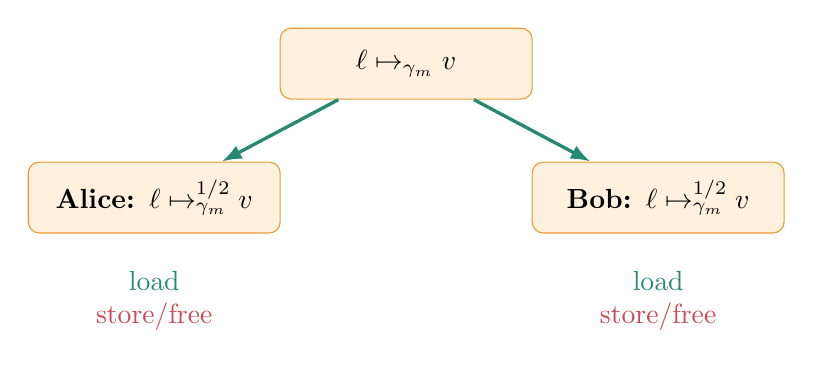
\begin{tikzpicture}[
    token/.style={rounded corners,draw=CrisAmber,fill=CrisLightAmber,minimum width=3.2cm,minimum height=0.9cm,align=center,font=\bfseries},
    arr/.style={-{Latex[length=2.5mm]},very thick,CrisGreen}
  ]
    \node[token] (full) at (0,1.3) {\(\ptfull{\ell}{v}\)};
    \node[token] (a) at (-3.2,-0.4) {Alice: \(\ptfrac{\ell}{1/2}{v}\)};
    \node[token] (b) at (3.2,-0.4) {Bob: \(\ptfrac{\ell}{1/2}{v}\)};
    \draw[arr] (full) -- (a);
    \draw[arr] (full) -- (b);
    \node[below=0.35cm of a,align=center] {\good{load}\\\warn{store/free}};
    \node[below=0.35cm of b,align=center] {\good{load}\\\warn{store/free}};
  \end{tikzpicture}
  \end{center}

  \vspace{0.3cm}
  \begin{block}{To write again}
    Recombine every outstanding share to recover fraction 1, then invoke the full-element update rule.
  \end{block}
\end{frame}

% 20 -- 54:00
\begin{frame}{A Rust analogy---and its boundary}
  \renewcommand{\arraystretch}{1.35}
  \begin{tabularx}{\textwidth}{X X}
    \toprule
    \textbf{Fractional permission story} & \textbf{Rust intuition} \\
    \midrule
    several proper fractions may read & several shared \texttt{\&T} borrows \\
    no proper fraction may write & shared aliases exclude mutable access \\
    recombine all shares to fraction 1 & all shared borrows have ended \\
    full token authorizes update & unique mutable access \\
    \bottomrule
  \end{tabularx}

  \vspace{0.7cm}
  \begin{alertblock}{Analogy, not a formal Rust model}
    \code{ghost_map} does not itself encode lexical lifetimes, reborrowing, compiler inference, or Rust's full type semantics.
  \end{alertblock}

  \begin{center}
    The useful common idea is: \keypoint{outstanding read shares prevent write authority}.
  \end{center}
\end{frame}

% 21 -- 56:00
\begin{frame}{Why a half-share cannot store}
  Suppose Alice and Bob each own a half-share asserting \(v\):
  \[
    \ptfrac{\ell}{1/2}{v}\Sep\ptfrac{\ell}{1/2}{v}.
  \]

  \vspace{0.25cm}
  If Alice alone changed her token to \(w\neq v\), Bob's compatible frame would remain:
  \[
    \colorbox{CrisLightRed}{\(\ptfrac{\ell}{1/2}{w}\Sep\ptfrac{\ell}{1/2}{v}\)}
    \qquad\warn{\text{invalid: same key, disagreeing values}.}
  \]

  \vspace{0.35cm}
  \begin{block}{Frame-preserving update test}
    A legal update must preserve validity with \emph{every} compatible environmental frame. Therefore no writer exists until all shares are recombined.
  \end{block}

  \begin{center}
    This matters even in a sequential program: Bob may be another module, callback, or later phase.
  \end{center}
\end{frame}

% 22 -- 58:00
\begin{frame}{DFrac adds persistent read-only knowledge}
  \begin{columns}[T,onlytextwidth]
    \column{0.42\textwidth}
      \begin{block}{Owned fraction}
        \[
          \ptfrac{\ell}{q}{v}
        \]
        Quantitative, splittable permission. Full fraction 1 is required for update/delete.
      \end{block}
    \column{0.42\textwidth}
      \begin{exampleblock}{Discarded knowledge}
        \[
          \ptro{\ell}{v}
        \]
        Persistent and freely duplicable. It records a permanently frozen value.
      \end{exampleblock}
  \end{columns}

  \vspace{0.45cm}
  \begin{center}
    \Large
    \(\ptfrac{\ell}{q}{v}\quad\upd\quad\ptro{\ell}{v}\)
  \end{center}

  \begin{alertblock}{What is discarded?}
    Discard the \emph{write capability}; retain duplicable knowledge of the value.
  \end{alertblock}

  \vfill
  \api{ghost_map_elem_persist}
\end{frame}

% 23 -- 60:00
\begin{frame}{Completion flag: update first, publish second}
  \begin{center}
  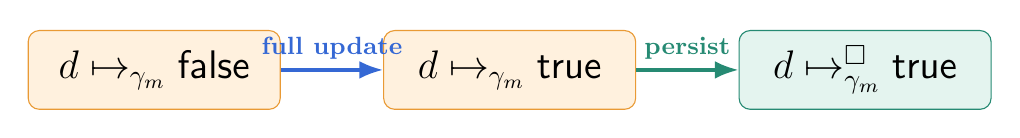
\begin{tikzpicture}[
    token/.style={rounded corners,draw,minimum width=3.2cm,minimum height=1.0cm,align=center,font=\Large},
    arr/.style={-{Latex[length=3mm]},very thick}
  ]
    \node[token,draw=CrisAmber,fill=CrisLightAmber] (f) {\(\ptfull{d}{\mathsf{false}}\)};
    \node[token,draw=CrisAmber,fill=CrisLightAmber,right=1.3cm of f] (t) {\(\ptfull{d}{\mathsf{true}}\)};
    \node[token,draw=CrisGreen,fill=CrisLightGreen,right=1.3cm of t] (p) {\(\ptro{d}{\mathsf{true}}\)};
    \draw[arr,CrisBlue] (f) -- node[above,font=\small\bfseries]{full update} (t);
    \draw[arr,CrisGreen] (t) -- node[above,font=\small\bfseries]{persist} (p);
  \end{tikzpicture}
  \end{center}

  \vspace{0.7cm}
  \begin{itemize}
    \item Before completion, full ownership authorizes the one update.
    \item After completion, persistent \(\mathsf{true}\) can be copied to any number of clients.
    \item The persistent frame prevents full write ownership from ever being recovered.
  \end{itemize}

  \begin{exampleblock}{Use case}
    Publish an initialized table, a completed task result, or finalized configuration as immutable knowledge.
  \end{exampleblock}
\end{frame}

% 24 -- 61:30
\begin{frame}{Persistence freezes the value you have \emph{now}}
  \begin{alertblock}{Wrong order}
    \[
      \ptfull{d}{\mathsf{false}}\upd\ptro{d}{\mathsf{false}}
    \]
    This freezes the flag at \(\mathsf{false}\). It does \emph{not} reserve a future transition to \(\mathsf{true}\).
  \end{alertblock}

  \vspace{0.35cm}
  \begin{block}{If observers need facts before the transition}
    Use a monotone / one-shot state-machine protocol. Encode \(\mathsf{false}<\mathsf{true}\), permit only upward movement, and publish a persistent completion witness afterward.
  \end{block}

  \vspace{0.2cm}
  \small
  Upstream Iris also provides \code{ghost_map_elem_unpersist}, but it yields only an unspecified fraction---never the full fraction needed to write while a persistent frame exists. (The current CRIS port leaves this lemma commented out.)
\end{frame}

% 25 -- 63:00
\begin{frame}{Checkpoint: classify the capability}
  \small
  \renewcommand{\arraystretch}{1.42}
  \begin{tabularx}{\textwidth}{>{\bfseries}l c c c c X}
    \toprule
    token & load & store/free & split & copy freely & intended reading \\
    \midrule
    full owned & \good{yes} & \good{yes} & \good{yes} & \warn{no} & mutable exclusive access \\
    proper fraction & \good{yes} & \warn{no} & \good{yes} & \warn{no} & shared read permission \\
    discarded / persistent & \good{yes} & \warn{no} & --- & \good{yes} & immutable published fact \\
    \bottomrule
  \end{tabularx}

  \vspace{0.55cm}
  \begin{exampleblock}{Quick retrieval questions}
    \begin{enumerate}
      \item Two components must read: which token shape?
      \item A component must store: what must be recombined?
      \item Everyone may retain the final value forever: which transition?
    \end{enumerate}
  \end{exampleblock}

  \scriptsize The standard \code{ghost_map} API directly supports persistent reads. The checked-in \code{MemA.load} is currently parameterized by an owned rational fraction.
\end{frame}

% 26 -- 66:00
\begin{frame}[fragile]{A benchmark across unknown code}
\begin{lstlisting}[style=criscode]
before = Mem.get_count();
f();                           // arbitrary; may call Mem
after = Mem.get_count();
assert(0 <= after - before);   // if f returns
\end{lstlisting}

  \begin{columns}[T,onlytextwidth]
    \column{0.47\textwidth}
      \begin{block}{Counter policy}
        Count completed \code{alloc/load/store/free} calls. Query itself does not increment.
      \end{block}
    \column{0.49\textwidth}
      \begin{alertblock}{Proof challenge}
        After \code{f}, we need a stable fact about an \emph{old} observation even though the current state may have changed.
      \end{alertblock}
  \end{columns}

  \vspace{0.25cm}
  \small Model the counter as an unbounded natural. A machine implementation must separately rule out wraparound or specify it.
\end{frame}

% 27 -- 69:00
\begin{frame}{A result-only query spec forgets history}
  A weak specification says only:
  \[
    \code{get\_count()}\quad\{\;\exists n.\ \mathsf{ret}=n\Sep\mathsf{Current}(n)\;\}.
  \]

  Calling it twice produces unrelated names:
  \[
    \exists n_0.\ \mathsf{before}=n_0
    \qquad\qquad
    \exists n_1.\ \mathsf{after}=n_1.
  \]

  \begin{alertblock}{Missing link}
    What connects \(n_0\) to \(n_1\) after arbitrary \code{f}? Exact current-state ownership cannot remain exact when the state changes.
  \end{alertblock}

  \begin{exampleblock}{Desired receipt}
    The first query should return a durable token \(\Snap{n_0}\): “the counter has reached at least \(n_0\).”
  \end{exampleblock}
\end{frame}

% 28 -- 71:00
\begin{frame}{\code{mono\_nat}: authority plus lower-bound snapshots}
  \begin{columns}[T,onlytextwidth]
    \column{0.40\textwidth}
      \begin{block}{Current authority}
        \[
          \AuthC{n}
        \]
        The module's exact current logical count.
      \end{block}
    \column{0.56\textwidth}
      \begin{exampleblock}{Past receipt}
        \[
          \Snap{m}
        \]
        Persistent claim: the current count is at least \(m\). It does not say the count remains exactly \(m\).
      \end{exampleblock}
  \end{columns}

  \vspace{0.25cm}
  \begin{center}
  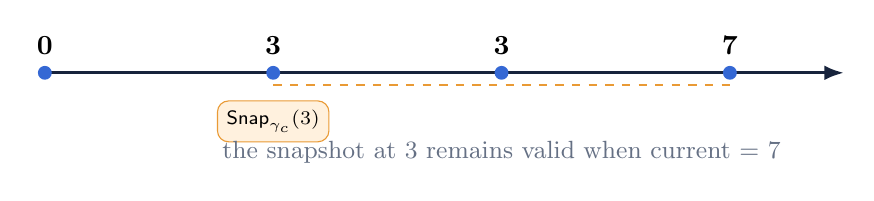
\begin{tikzpicture}[x=1.45cm,y=1cm]
    \draw[-{Latex[length=2.5mm]},very thick,CrisNavy] (0,0)--(7,0);
    \foreach \x/\n in {0/0,2/3,4/3,6/7}{
      \fill[CrisBlue] (\x,0) circle (2.5pt);
      \node[above=3pt,font=\bfseries] at (\x,0) {\n};
    }
    \node[draw=CrisAmber,fill=CrisLightAmber,rounded corners,below=0.35cm] at (2,0) {\scriptsize \(\Snap{3}\)};
    \draw[CrisAmber,dashed,thick] (2,-0.15)--(6,-0.15);
    \node[below=0.75cm,font=\small,CrisMuted] at (4,0) {the snapshot at 3 remains valid when current = 7};
  \end{tikzpicture}
  \end{center}

  \scriptsize “Snapshot” is presentation terminology; the installed proposition is \code{mono_nat_lb_own}.
\end{frame}

% 29 -- 74:00
\begin{frame}{Three rules prove the monotone protocol}
  \renewcommand{\arraystretch}{1.55}
  \begin{tabularx}{\textwidth}{>{\bfseries}l X}
    snapshot & \(\AuthC{n}\quad\Longrightarrow\quad\Snap{n}\) \\
    increase & \(\AuthC{n}\Sep\ulcorner n\le n'\urcorner\quad\upd\quad\AuthC{n'}\Sep\Snap{n'}\) \\
    validity & \(\AuthC{n}\Sep\Snap{m}\quad\Longrightarrow\quad\ulcorner m\le n\urcorner\) \\
  \end{tabularx}

  \vspace{0.45cm}
  \begin{center}
    \api{mono_nat_lb_own_get}\qquad
    \api{mono_nat_own_update}\qquad
    \api{mono_nat_lb_own_valid}
  \end{center}

  \scriptsize These are the exact upstream Iris names. A CRIS implementation needs a small \code{CRIS.own} wrapper; this checkout has no local \code{mono_nat.v} port yet.

  \begin{block}{Compare the validity relations}
    \code{ghost_map}: element and authority agree on an \keypoint{exact value}.\\
    \code{mono_nat}: snapshot and authority agree through the \keypoint{order} \(m\le n\).
  \end{block}
\end{frame}

% 30 -- 78:00
\begin{frame}{Compose both protocols inside one IST}
  \small
  \begin{block}{Simplified combined invariant}
  \[
  \begin{aligned}
  \mathsf{IST}\triangleq\exists m,M,c,n.\quad
    &\ulcorner\mathsf{concrete\_heap}=m\land\mathsf{repr}(m)=M\urcorner \\
    &{}\Sep \AuthM{M} \\
    &{}\Sep \ulcorner\mathsf{concrete\_count}=c\land c=n\urcorner \\
    &{}\Sep \AuthC{n}.
  \end{aligned}
  \]
  \end{block}

  \begin{columns}[T,onlytextwidth]
    \column{0.47\textwidth}
      \begin{exampleblock}{Memory protocol}
        Update only the owned key; frame all other element resources.
      \end{exampleblock}
    \column{0.49\textwidth}
      \begin{exampleblock}{Counter protocol}
        Each counted operation moves \(n\) to \(n+1\) before reclosing the IST.
      \end{exampleblock}
  \end{columns}

  \begin{center}
    Independent protocols compose with separating conjunction / a product RA.
  \end{center}
\end{frame}

% 31 -- 80:00
\begin{frame}{Query spec: supply a past lower bound}
  The program has no argument. Its \emph{specification} is parameterized by a prior observation \(m\):

  \vspace{0.3cm}
  \begin{block}{\code{get_count()} for any ghost parameter \(m\)}
    \[
      \underbrace{\Snap{m}}_{\text{pre}}
      \quad\Longrightarrow\quad
      \exists n.\;
        \underbrace{\ulcorner\mathsf{ret}=n\land m\le n\urcorner\Sep\Snap{n}}_{\text{post}}.
    \]
  \end{block}

  \begin{enumerate}
    \item Open the IST and obtain exact authority \(\AuthC{n}\).
    \item Validity with \(\Snap{m}\) gives \(m\le n\).
    \item Snapshot the current \(n\), return the concrete value, and reclose the IST.
  \end{enumerate}

  \small Because \(\Snap{m}\) is persistent, the caller may retain and reuse it. Initialization supplies \(\Snap{0}\).
\end{frame}

% 32 -- 82:00
\begin{frame}{The complete client proof}
  \begin{center}
  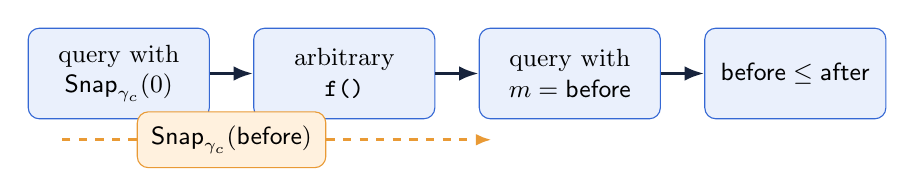
\begin{tikzpicture}[
    stage/.style={rounded corners,draw=CrisBlue,fill=CrisLightBlue,minimum width=2.3cm,minimum height=1.15cm,align=center,font=\small},
    token/.style={rounded corners,draw=CrisAmber,fill=CrisLightAmber,inner sep=5pt,font=\small\bfseries},
    arr/.style={-{Latex[length=2.5mm]},very thick,CrisNavy}
  ]
    \node[stage] (q0) {query with\\\(\Snap{0}\)};
    \node[stage,right=0.55cm of q0] (f) {arbitrary\\\code{f()}};
    \node[stage,right=0.55cm of f] (q1) {query with\\\(m=\mathsf{before}\)};
    \node[stage,right=0.55cm of q1] (res) {\(\mathsf{before}\le\mathsf{after}\)};
    \draw[arr] (q0)--(f); \draw[arr] (f)--(q1); \draw[arr] (q1)--(res);
    \node[token,below=0.48cm of $(q0)!0.5!(f)$] (snap) {\(\Snap{\mathsf{before}}\)};
    \draw[CrisAmber,very thick,dashed] (snap.west) -- ++(-1.05,0);
    \draw[CrisAmber,very thick,dashed,-{Latex[length=2mm]}] (snap.east) -- ++(2.1,0);
  \end{tikzpicture}
  \end{center}

  \vspace{0.45cm}
  \begin{enumerate}
    \item First query returns \(\mathsf{before}\) and a persistent snapshot of it.
    \item Carry the snapshot across \code{f}; no functional spec for \code{f} is needed.
    \item Instantiate the second query's ghost parameter with \(\mathsf{before}\).
    \item Its postcondition gives \(\mathsf{before}\le\mathsf{after}\).
    \item Over integers: \(0\le(\mathsf{after}:\mathbb Z)-(\mathsf{before}:\mathbb Z)\).
  \end{enumerate}
\end{frame}

% 33 -- 84:00
\begin{frame}{What arbitrary \code{f} can---and cannot---do}
  \begin{columns}[T,onlytextwidth]
    \column{0.47\textwidth}
      \begin{exampleblock}{May do}
        \begin{itemize}
          \item call public memory operations,
          \item perform any number of accesses,
          \item return any value or perform I/O,
          \item diverge.
        \end{itemize}
      \end{exampleblock}
    \column{0.49\textwidth}
      \begin{alertblock}{Cannot do}
        \begin{itemize}
          \item directly mutate scoped private counter state,
          \item forge the hidden full authority,
          \item make a verified public method move authority downward.
        \end{itemize}
      \end{alertblock}
  \end{columns}

  \vspace{0.45cm}
  \begin{block}{Precise claim}
    If \code{f} and the second query return, then \(\mathsf{before}\le\mathsf{after}\). This is robustness to unknown functional behavior, not a termination proof for \code{f}.
  \end{block}
\end{frame}

% 34 -- 85:00
\begin{frame}{Choose an RA by asking what must remain compatible}
  \small
  \renewcommand{\arraystretch}{1.28}
  \begin{tabularx}{\textwidth}{X X}
    \toprule
    \textbf{Program protocol} & \textbf{Useful library shape} \\
    \midrule
    stable agreement on a value & \code{agree} \\
    unique, nonduplicable capability & \code{excl} \\
    central truth plus client views & \code{auth} \\
    independently owned keyed entries & \code{ghost_map} \\
    increasing natural / integer & \code{mono_nat} / \code{mono_Z} \\
    append-only history; prefix snapshots & \code{mono_list} \\
    \bottomrule
  \end{tabularx}

  \vspace{0.45cm}
  \begin{center}
    \Large\bfseries\color{CrisNavy}
    The RA operation and validity relation implement the protocol.
  \end{center}

  \small Upstream Iris provides these algebra libraries. CRIS already ports \code{ghost_map} and \code{mono_list}; a matching local \code{mono_nat} wrapper remains to be added.
\end{frame}

% 35 -- 87:00
\begin{frame}{A four-question design recipe}
  \begin{enumerate}
    \item \textbf{Private state:} what concrete state must the module protect?
    \item \textbf{Client view:} what capability or durable fact should cross the API boundary?
    \item \textbf{Compatibility:} which simultaneous client claims may coexist?
    \item \textbf{Evolution:} which updates must preserve all compatible frames?
  \end{enumerate}

  \vspace{0.45cm}
  \begin{center}
  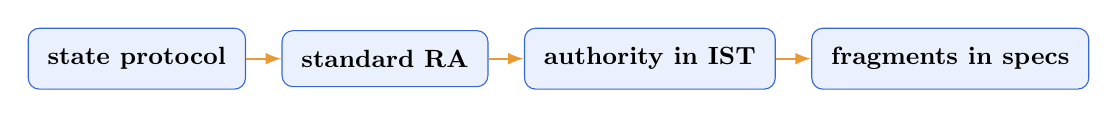
\begin{tikzpicture}[
    node distance=0.45cm,
    box/.style={rounded corners,draw=CrisBlue,fill=CrisLightBlue,inner sep=7pt,font=\small\bfseries},
    arr/.style={-{Latex[length=2mm]},CrisAmber,thick}
  ]
    \node[box] (p) {state protocol};
    \node[box,right=of p] (ra) {standard RA};
    \node[box,right=of ra] (ist) {authority in IST};
    \node[box,right=of ist] (api) {fragments in specs};
    \draw[arr] (p)--(ra); \draw[arr] (ra)--(ist); \draw[arr] (ist)--(api);
  \end{tikzpicture}
  \end{center}

  \begin{block}{Composition}
    A module may enforce several independent protocols at once by combining their resources with a product / separating conjunction.
  \end{block}
\end{frame}

% 36 -- 88:30
\begin{frame}{Three rules to take to the afternoon}
  \begin{block}{1. Exact lookup}
    \[
      \AuthM{M}\Sep\ptfrac{\ell}{q}{v}\quad\Longrightarrow\quad M(\ell)=v
    \]
  \end{block}
  \begin{block}{2. Permission accounting}
    \[
      \text{full element}\Rightarrow\text{update/free}
      \qquad
      \text{fraction}\Rightarrow\text{read}
    \]
  \end{block}
  \begin{block}{3. Past versus current}
    \[
      \AuthC{n}\Sep\Snap{m}\quad\Longrightarrow\quad m\le n
    \]
  \end{block}

  \begin{center}
    \Large\bfseries\color{CrisNavy}
    Resources are executable proof protocols for modular clients.
  \end{center}
\end{frame}

% -------------------------- Backup slides --------------------------

\begin{frame}{Backup: current artifact vs. \texorpdfstring{\texttt{ghost\_map}}{ghost_map}}
  \small
  \renewcommand{\arraystretch}{1.28}
  \begin{tabularx}{\textwidth}{>{\raggedright\arraybackslash}X >{\raggedright\arraybackslash}X}
    \toprule
    \textbf{Current \code{imp_system/mem}} & \textbf{Standard-library presentation} \\
    \midrule
    nested discrete functions + \code{optionUR} + \code{dfrac_agreeR} & \code{ghost_mapG} hides \code{gmap_viewR} \\
    \code{own mem_name (● mem_src)} & \code{ghost_map_auth gamma 1 M} \\
    \code{mem_points_to_singleton} & \code{ghost_map_elem gamma l dq v} \\
    \code{mem_ra_lookup} & \code{ghost_map_lookup} \\
    \code{mem_ra_update} & \code{ghost_map_update} \\
    \code{mem_ra_free} & \code{ghost_map_delete} \\
    \code{mem_ra_alloc} & \code{ghost_map_insert(_big)} \\
    \bottomrule
  \end{tabularx}

  \vspace{0.45cm}
  \begin{block}{Why teach the library version?}
    It exposes the reusable protocol and avoids making the first encounter depend on implementation details of the camera carrier.
  \end{block}
\end{frame}

\begin{frame}[fragile]{Backup: exact installed \code{ghost_map} API}
\begin{lstlisting}[style=criscode,basicstyle=\ttfamily\scriptsize]
ghost_map_auth gamma q m
ghost_map_elem gamma k (DfracOwn q) v
ghost_map_elem gamma k (DfracOwn 1) v
ghost_map_elem gamma k DfracDiscarded v

ghost_map_lookup
ghost_map_insert
ghost_map_update
ghost_map_delete
ghost_map_elem_persist
\end{lstlisting}

  \small
  Source: \code{_opam/lib/coq/user-contrib/iris/base_logic/lib/ghost_map.v}.
  Definitions/notation: lines 28--49; fractions/persistence: 62--69 and 136--150;
  lookup/update rules: 221--279. CRIS's main compatibility port is at
  \code{CRIS/theories/iris_system/lib/ghost_map.v}.
\end{frame}

\begin{frame}[fragile]{Backup: the checked-in core memory specs}
\begin{lstlisting}[style=criscode,basicstyle=\ttfamily\scriptsize]
alloc:  ret = Vptr (b,0)
        * (b,0) |-> replicate sz Vundef

load:   (b,ofs) |->{q} v
        ==> ret = v * (b,ofs) |->{q} v

store:  (b,ofs) |-> v_old
        ==> ret = 0 * (b,ofs) |-> v_new

free:   (b,ofs) |-> v
        ==> ret = 0
\end{lstlisting}

  \small Source: \code{imp_system/mem/MemA.v:220--239}. The implementation also exports compare and CAS; omit them from the first explanation.
\end{frame}

\begin{frame}[fragile]{Backup: exact installed \code{mono_nat} API}
\begin{lstlisting}[style=criscode,basicstyle=\ttfamily\scriptsize]
mono_nat_auth_own gamma q n       (* exact authority *)
mono_nat_lb_own gamma m           (* persistent lower bound *)

mono_nat_lb_own_get           (* auth n -> lower bound n *)
mono_nat_own_update           (* n <= n' -> update auth *)
mono_nat_lb_own_valid         (* auth n + lb m -> m <= n *)
\end{lstlisting}

  \small
  Source: \code{_opam/lib/coq/user-contrib/iris/base_logic/lib/mono_nat.v}.
  The header uses stale shorthand names in prose; the identifiers above are the actual definitions in this checkout.
  They require a small adapter to CRIS's non-step-indexed \code{own} before use in a CRIS IST.
\end{frame}

\begin{frame}{Backup: access-counter engineering choices}
  \renewcommand{\arraystretch}{1.3}
  \begin{tabularx}{\textwidth}{>{\bfseries}l X}
    \toprule
    choice & consequence \\
    \midrule
    Does query count? & Monotonicity survives either choice; benchmark overhead and interpretation differ. \\
    What counts as access? & Fix alloc/load/store/free, or just load/store, before writing the specs. \\
    What about CAS? & Count one public CAS or count its internal load/store calls---but state which. \\
    Machine overflow? & Exclude it, saturate, use unbounded runtime integers, or weaken the abstraction to modular behavior. \\
    What if \code{f} diverges? & No second query; the post-return inequality is not a termination claim. \\
    \bottomrule
  \end{tabularx}
\end{frame}

\begin{frame}{Backup: DFrac has a third internal shape}
  \begin{itemize}
    \item \code{DfracOwn q}: own quantitative fraction \(q\).
    \item \code{DfracDiscarded}: know that a fraction was discarded; persistent.
    \item \code{DfracBoth q}: own \(q\) and know some fraction was discarded.
  \end{itemize}

  \vspace{0.4cm}
  \[
    \mathsf{DfracBoth}(q)
    = \mathsf{DfracOwn}(q)\cdot\mathsf{DfracDiscarded}
  \]

  \begin{block}{Why it matters}
    Once discarded knowledge exists, validity requires owned fractions to total strictly less than 1. Therefore nobody can hold full write authority now or in the future.
  \end{block}

  \small Source: \code{iris/algebra/dfrac.v:1--20, 26--106}.
\end{frame}

\begin{frame}{Backup: the paper's hybrid memory is a different point}
  \begin{block}{Section 7 / Figure 12}
    The paper's hybrid specification uses \code{take} so a client proof may select either:
    \begin{itemize}
      \item an ownership-based memory specification, or
      \item a concrete operational memory model with nondeterministic allocation.
    \end{itemize}
  \end{block}

  \begin{alertblock}{Do not conflate the examples}
    Today's \code{ghost_map} story asks how to implement the ownership protocol cleanly. The paper's example asks how an imaginary specification can offer ownership and operational reasoning as alternative branches.
  \end{alertblock}
\end{frame}

\begin{frame}{Backup: source anchors for the mechanized store proof}
  \small
  \begin{itemize}
    \item Concrete \code{SGet}/\code{SPut} store: \code{MemI.v:111--117}.
    \item Public full-ownership store spec: \code{MemA.v:235--238}.
    \item Logical/concrete heap relation: \code{MemIAproof.v:9--13}.
    \item IST with full authoritative ownership: \code{MemIAproof.v:224--228}.
    \item Lookup lemma: \code{MemIAproof.v:116--138}.
    \item Joint authority/fragment update: \code{MemIAproof.v:140--162}.
    \item Store simulation: \code{MemIAproof.v:325--346}.
  \end{itemize}

  \begin{exampleblock}{Reading strategy}
    Align the proof script with the five conceptual steps on Slide 16. Treat tactics as bookkeeping around the same resource transition.
  \end{exampleblock}
\end{frame}

\end{document}
